% Options for packages loaded elsewhere
\PassOptionsToPackage{unicode}{hyperref}
\PassOptionsToPackage{hyphens}{url}
%
\documentclass[
]{article}
\usepackage{amsmath,amssymb}
\usepackage{lmodern}
\usepackage{ifxetex,ifluatex}
\ifnum 0\ifxetex 1\fi\ifluatex 1\fi=0 % if pdftex
  \usepackage[T1]{fontenc}
  \usepackage[utf8]{inputenc}
  \usepackage{textcomp} % provide euro and other symbols
\else % if luatex or xetex
  \usepackage{unicode-math}
  \defaultfontfeatures{Scale=MatchLowercase}
  \defaultfontfeatures[\rmfamily]{Ligatures=TeX,Scale=1}
\fi
% Use upquote if available, for straight quotes in verbatim environments
\IfFileExists{upquote.sty}{\usepackage{upquote}}{}
\IfFileExists{microtype.sty}{% use microtype if available
  \usepackage[]{microtype}
  \UseMicrotypeSet[protrusion]{basicmath} % disable protrusion for tt fonts
}{}
\makeatletter
\@ifundefined{KOMAClassName}{% if non-KOMA class
  \IfFileExists{parskip.sty}{%
    \usepackage{parskip}
  }{% else
    \setlength{\parindent}{0pt}
    \setlength{\parskip}{6pt plus 2pt minus 1pt}}
}{% if KOMA class
  \KOMAoptions{parskip=half}}
\makeatother
\usepackage{xcolor}
\IfFileExists{xurl.sty}{\usepackage{xurl}}{} % add URL line breaks if available
\IfFileExists{bookmark.sty}{\usepackage{bookmark}}{\usepackage{hyperref}}
\hypersetup{
  pdftitle={Stat 230 HW 6},
  pdfauthor={Name: Victor Huang},
  hidelinks,
  pdfcreator={LaTeX via pandoc}}
\urlstyle{same} % disable monospaced font for URLs
\usepackage[margin=1in]{geometry}
\usepackage{color}
\usepackage{fancyvrb}
\newcommand{\VerbBar}{|}
\newcommand{\VERB}{\Verb[commandchars=\\\{\}]}
\DefineVerbatimEnvironment{Highlighting}{Verbatim}{commandchars=\\\{\}}
% Add ',fontsize=\small' for more characters per line
\usepackage{framed}
\definecolor{shadecolor}{RGB}{248,248,248}
\newenvironment{Shaded}{\begin{snugshade}}{\end{snugshade}}
\newcommand{\AlertTok}[1]{\textcolor[rgb]{0.94,0.16,0.16}{#1}}
\newcommand{\AnnotationTok}[1]{\textcolor[rgb]{0.56,0.35,0.01}{\textbf{\textit{#1}}}}
\newcommand{\AttributeTok}[1]{\textcolor[rgb]{0.77,0.63,0.00}{#1}}
\newcommand{\BaseNTok}[1]{\textcolor[rgb]{0.00,0.00,0.81}{#1}}
\newcommand{\BuiltInTok}[1]{#1}
\newcommand{\CharTok}[1]{\textcolor[rgb]{0.31,0.60,0.02}{#1}}
\newcommand{\CommentTok}[1]{\textcolor[rgb]{0.56,0.35,0.01}{\textit{#1}}}
\newcommand{\CommentVarTok}[1]{\textcolor[rgb]{0.56,0.35,0.01}{\textbf{\textit{#1}}}}
\newcommand{\ConstantTok}[1]{\textcolor[rgb]{0.00,0.00,0.00}{#1}}
\newcommand{\ControlFlowTok}[1]{\textcolor[rgb]{0.13,0.29,0.53}{\textbf{#1}}}
\newcommand{\DataTypeTok}[1]{\textcolor[rgb]{0.13,0.29,0.53}{#1}}
\newcommand{\DecValTok}[1]{\textcolor[rgb]{0.00,0.00,0.81}{#1}}
\newcommand{\DocumentationTok}[1]{\textcolor[rgb]{0.56,0.35,0.01}{\textbf{\textit{#1}}}}
\newcommand{\ErrorTok}[1]{\textcolor[rgb]{0.64,0.00,0.00}{\textbf{#1}}}
\newcommand{\ExtensionTok}[1]{#1}
\newcommand{\FloatTok}[1]{\textcolor[rgb]{0.00,0.00,0.81}{#1}}
\newcommand{\FunctionTok}[1]{\textcolor[rgb]{0.00,0.00,0.00}{#1}}
\newcommand{\ImportTok}[1]{#1}
\newcommand{\InformationTok}[1]{\textcolor[rgb]{0.56,0.35,0.01}{\textbf{\textit{#1}}}}
\newcommand{\KeywordTok}[1]{\textcolor[rgb]{0.13,0.29,0.53}{\textbf{#1}}}
\newcommand{\NormalTok}[1]{#1}
\newcommand{\OperatorTok}[1]{\textcolor[rgb]{0.81,0.36,0.00}{\textbf{#1}}}
\newcommand{\OtherTok}[1]{\textcolor[rgb]{0.56,0.35,0.01}{#1}}
\newcommand{\PreprocessorTok}[1]{\textcolor[rgb]{0.56,0.35,0.01}{\textit{#1}}}
\newcommand{\RegionMarkerTok}[1]{#1}
\newcommand{\SpecialCharTok}[1]{\textcolor[rgb]{0.00,0.00,0.00}{#1}}
\newcommand{\SpecialStringTok}[1]{\textcolor[rgb]{0.31,0.60,0.02}{#1}}
\newcommand{\StringTok}[1]{\textcolor[rgb]{0.31,0.60,0.02}{#1}}
\newcommand{\VariableTok}[1]{\textcolor[rgb]{0.00,0.00,0.00}{#1}}
\newcommand{\VerbatimStringTok}[1]{\textcolor[rgb]{0.31,0.60,0.02}{#1}}
\newcommand{\WarningTok}[1]{\textcolor[rgb]{0.56,0.35,0.01}{\textbf{\textit{#1}}}}
\usepackage{graphicx}
\makeatletter
\def\maxwidth{\ifdim\Gin@nat@width>\linewidth\linewidth\else\Gin@nat@width\fi}
\def\maxheight{\ifdim\Gin@nat@height>\textheight\textheight\else\Gin@nat@height\fi}
\makeatother
% Scale images if necessary, so that they will not overflow the page
% margins by default, and it is still possible to overwrite the defaults
% using explicit options in \includegraphics[width, height, ...]{}
\setkeys{Gin}{width=\maxwidth,height=\maxheight,keepaspectratio}
% Set default figure placement to htbp
\makeatletter
\def\fps@figure{htbp}
\makeatother
\setlength{\emergencystretch}{3em} % prevent overfull lines
\providecommand{\tightlist}{%
  \setlength{\itemsep}{0pt}\setlength{\parskip}{0pt}}
\setcounter{secnumdepth}{-\maxdimen} % remove section numbering
\ifluatex
  \usepackage{selnolig}  % disable illegal ligatures
\fi

\title{Stat 230 HW 6}
\author{Name: Victor Huang}
\date{}

\begin{document}
\maketitle

\hypertarget{worked-with-no-one}{%
\subsubsection{worked with: No one}\label{worked-with-no-one}}

Homework 6 is due \textbf{by 3pm Thursday, Oct.~4}. Please complete the
assignment in this Markdown document, filling in your answers and R code
below. I didn't create answer and R chunk fields like I did with
homework 1, but please fill in your answers and R code in the same
manner as hw 1. Submit a hard copy of the \textbf{compiled pdf or word
doc} either

\begin{itemize}
\tightlist
\item
  in class
\item
  in drop-in office hours
\item
  in the paper holder outside my CMC 222 office door
\end{itemize}

Tips for using Markdown with homework sets:

\begin{itemize}
\tightlist
\item
  Work through a problem by putting your R code into R chunks in this
  .Rmd. Run the R code to make sure it works, then knit the .Rmd to
  verify they work in that environment.

  \begin{itemize}
  \tightlist
  \item
    Make sure you load your data in the .Rmd and include any needed
    \texttt{library} commands.
  \end{itemize}
\item
  Feel free to edit or delete questions, instructions, or code provided
  in this file when producing your homework solution.
\item
  For your final document, you can change the output type from
  \texttt{html\_document} to \texttt{word\_document} or
  \texttt{pdf\_document}. These two to output types are better formatted
  for printing.

  \begin{itemize}
  \tightlist
  \item
    on maize: you may need to allow for pop-ups from this site
  \end{itemize}
\item
  If you want to knit to pdf while running Rstudio from your computer
  (\emph{not} from maize), you will need a LaTeX compiler installed on
  your computer. This could be \href{https://miktex.org/}{MiKTeX},
  \href{http://www.tug.org/mactex/}{MacTeX} (mac), or TinyTex. The
  latter is installed in R: first install the R package
  \texttt{tinytex}, then run the command
  \texttt{tinytex::install\_tinytex()} to install this software.

  \begin{itemize}
  \tightlist
  \item
    If you are using maize, you don't need to install anything to knit
    to pdf!
  \end{itemize}
\end{itemize}

\begin{center}\rule{0.5\linewidth}{0.5pt}\end{center}

\hypertarget{problem-1-donner-ch.20-exercise-9}{%
\subsection{Problem 1: Donner Ch.20 Exercise
9}\label{problem-1-donner-ch.20-exercise-9}}

Just use the estimated log odds model \textbf{given in this exercise} to
answer the question ``by hand'' (\emph{don't} fit the model in R and use
the predict command). \textbf{Show all formulas and worked needed to
derive your answers.}

\begin{enumerate}
\def\labelenumi{\alph{enumi}.}
\tightlist
\item
  \[
  logodds_{females} = 3.2 - 0.078(age),logodds_{males} = 1.6 - 0.078(age)
  \]
  \(\hat \pi(females = 25) = \frac{e^{3.2 - 0.078(25)}}{1 + e^{3.2 - 0.078(25)}} = 0.777\)
  \newline
  \(\hat \pi(males = 25) = \frac{e^{1.6 - 0.078(25)}}{1 + e^{1.6 - 0.078(25)}} = 0.413\)
  \newline
  \(\hat \pi(females = 50) = \frac{e^{3.2 - 0.078(50)}}{1 + e^{3.2 - 0.078(50)}} = 0.332\)
  \newline
  \(\hat \pi(males = 50) = \frac{e^{1.6 - 0.078(50)}}{1 + e^{1.6 - 0.078(50)}} = 0.091\)
  \newline \newline
\item
  \(\frac{e^{3.2 - 0.078(age)}}{1 + e^{3.2 - 0.078(age)}} = 0.5\)
  \newline \(e^{3.2 - 0.078(age)} = 1\) (to get \(\frac{1}{2}\) we have
  to make sure the denominator is two and the numerator is 1. As such,
  we can set the \(\hat \pi\) term equal to 1) \newline
  \(3.2 - 0.078(age) = ln(1)\) \newline \(-0.078(age) = 0 - 3.2\)
  \newline \(-0.078(age) = -3.2\) \newline \(age = \frac{-3.2}{-0.078}\)
  \newline \(age = 41\) (females) \newline \newline
  \(\frac{e^{1.6 - 0.078(age)}}{1 + e^{1.6 - 0.078(age)}} = 0.5\)
  \newline \(e^{1.6 - 0.078(age)} = 1\) (to get \(\frac{1}{2}\) we have
  to make sure the denominator is two and the numerator is 1. As such,
  we can set the \(\hat \pi\) term equal to 1) \newline
  \(1.6 - 0.078(age) = ln(1)\) \newline \(-0.078(age) = 0 - 1.6\)
  \newline \(-0.078(age) = -1.6\) \newline \(age = \frac{-1.6}{-0.078}\)
  \newline \(age = 20.5 \approx 21\) (males) \newline
\end{enumerate}

\begin{center}\rule{0.5\linewidth}{0.5pt}\end{center}

\hypertarget{problem-2-donner-interaction}{%
\subsection{Problem 2: Donner
interaction}\label{problem-2-donner-interaction}}

A comment in section 20.6.1 suggests that there may be a weak
interaction between sex and age in the donner data. Let's explore that
further. The data for this example is \texttt{case2001}.

\hypertarget{a-use-ggplot2-to-create-a-boxplot-of-age-by-status-that-is-faceted-by-sex.-explain-why-this-graph-is-suggestive-of-a-possible-interactive-effect-of-sex-and-age.}{%
\subsubsection{\texorpdfstring{(2a) Use \texttt{ggplot2} to create a
boxplot of \texttt{Age} by \texttt{Status} that is faceted by
\texttt{Sex}. Explain why this graph is suggestive of a possible
interactive effect of \texttt{Sex} and
\texttt{Age}.}{(2a) Use ggplot2 to create a boxplot of Age by Status that is faceted by Sex. Explain why this graph is suggestive of a possible interactive effect of Sex and Age.}}\label{a-use-ggplot2-to-create-a-boxplot-of-age-by-status-that-is-faceted-by-sex.-explain-why-this-graph-is-suggestive-of-a-possible-interactive-effect-of-sex-and-age.}}

\begin{Shaded}
\begin{Highlighting}[]
\NormalTok{case2001 }\OtherTok{=}\NormalTok{ case2001}
\FunctionTok{library}\NormalTok{(ggplot2)}
\FunctionTok{ggplot}\NormalTok{(case2001, }\FunctionTok{aes}\NormalTok{(}\AttributeTok{x =}\NormalTok{ Status, }\AttributeTok{y =}\NormalTok{ Age)) }\SpecialCharTok{+}
 \FunctionTok{geom\_boxplot}\NormalTok{() }\SpecialCharTok{+}
\FunctionTok{facet\_wrap}\NormalTok{(}\SpecialCharTok{\textasciitilde{}}\NormalTok{Sex) }\SpecialCharTok{+} 
 \FunctionTok{coord\_flip}\NormalTok{()}
\end{Highlighting}
\end{Shaded}

\includegraphics{homework6_files/figure-latex/unnamed-chunk-2-1.pdf}
Looking at the pair of boxplots above, we can clearly see that there is
a difference between the average death age for males and female with the
average male death age being approx. 28 years old and the average female
death age being approx. 45 years old (there is a larger gap between in
age of survived and age of dead for females and male). This would be
explained by the existence of and interactive effect between Sex and
Age.

\hypertarget{b-fit-the-logistic-regression-of-survival-status-on-age-sex-and-the-interaction-of-age-and-sex.-give-the-estimated-effect-for-the-interaction-and-the-p-value-based-on-the-wald-z-test-for-the-interaction-term.}{%
\subsubsection{(2b) Fit the logistic regression of survival status on
age, sex and the interaction of age and sex. Give the estimated effect
for the interaction and the p-value (based on the Wald z test) for the
interaction
term.}\label{b-fit-the-logistic-regression-of-survival-status-on-age-sex-and-the-interaction-of-age-and-sex.-give-the-estimated-effect-for-the-interaction-and-the-p-value-based-on-the-wald-z-test-for-the-interaction-term.}}

\begin{Shaded}
\begin{Highlighting}[]
\NormalTok{case2001\_glm }\OtherTok{\textless{}{-}} \FunctionTok{glm}\NormalTok{(Status }\SpecialCharTok{\textasciitilde{}}\NormalTok{ Age}\SpecialCharTok{*}\NormalTok{Sex, }\AttributeTok{family =}\NormalTok{ binomial, }\AttributeTok{data =}\NormalTok{ case2001)}
\FunctionTok{tidy}\NormalTok{(case2001\_glm)}
\CommentTok{\# A tibble: 4 x 5}
\NormalTok{  term        estimate std.error statistic p.value}
  \SpecialCharTok{\textless{}}\NormalTok{chr}\SpecialCharTok{\textgreater{}}          \ErrorTok{\textless{}}\NormalTok{dbl}\SpecialCharTok{\textgreater{}}     \ErrorTok{\textless{}}\NormalTok{dbl}\SpecialCharTok{\textgreater{}}     \ErrorTok{\textless{}}\NormalTok{dbl}\SpecialCharTok{\textgreater{}}   \ErrorTok{\textless{}}\NormalTok{dbl}\SpecialCharTok{\textgreater{}}
\DecValTok{1}\NormalTok{ (Intercept)    }\FloatTok{7.25}     \FloatTok{3.21}        \FloatTok{2.26}  \FloatTok{0.0238}
\DecValTok{2}\NormalTok{ Age           }\SpecialCharTok{{-}}\FloatTok{0.194}    \FloatTok{0.0874}     \SpecialCharTok{{-}}\FloatTok{2.22}  \FloatTok{0.0264}
\DecValTok{3}\NormalTok{ SexMale       }\SpecialCharTok{{-}}\FloatTok{6.93}     \FloatTok{3.40}       \SpecialCharTok{{-}}\FloatTok{2.04}  \FloatTok{0.0415}
\DecValTok{4}\NormalTok{ Age}\SpecialCharTok{:}\NormalTok{SexMale    }\FloatTok{0.162}    \FloatTok{0.0943}      \FloatTok{1.71}  \FloatTok{0.0865}
\end{Highlighting}
\end{Shaded}

\(\hat \eta = 7.2463848 - 0.1940741(Age) - 6.9280495(SexMale) + 0.1615969(Age)(SexMale)\)
\newline \(H_{0}: \beta_{3} = 0; H_{A}: \beta_{3} \neq 0}\) \newline
\(z-stat = \frac{0.1615969 - 0}{0.09426191} = 1.714339\)
\(p-value = 2 * P(Z < -1.714339) = 0.08646648\)

\begin{Shaded}
\begin{Highlighting}[]
\DecValTok{2}\SpecialCharTok{*}\FunctionTok{pnorm}\NormalTok{(}\SpecialCharTok{{-}}\FloatTok{1.714339}\NormalTok{)}
\NormalTok{[}\DecValTok{1}\NormalTok{] }\FloatTok{0.08646648}
\end{Highlighting}
\end{Shaded}

We get an estimated effect of 0.1615969, after going through the
calculations shown above, we get a p-value of 0.08646648.

\hypertarget{c-conduct-a-drop-in-deviance-test-for-the-interaction-term.-give-the-p-value-for-this-test-and-compare-it-to-the-wald-test-p-value.-does-you-conclusion-about-the-significance-of-the-interaction-term-change-explain.-moral-as-noted-in-comment-1-on-pages-616-617-you-should-trust-the-drop-in-deviance-test-more-than-the-wald-test.}{%
\subsubsection{(2c) Conduct a drop-in-deviance test for the interaction
term. Give the p-value for this test and compare it to the Wald test
p-value. Does you conclusion about the significance of the interaction
term change? Explain. (Moral: as noted in comment 1 on pages 616-617,
you should trust the drop in deviance test more than the Wald
test.)}\label{c-conduct-a-drop-in-deviance-test-for-the-interaction-term.-give-the-p-value-for-this-test-and-compare-it-to-the-wald-test-p-value.-does-you-conclusion-about-the-significance-of-the-interaction-term-change-explain.-moral-as-noted-in-comment-1-on-pages-616-617-you-should-trust-the-drop-in-deviance-test-more-than-the-wald-test.}}

\(H_{0}: \hat \eta = 7.2463848 - 0.1940741(Age) - 6.9280495(SexMale); H_{A}: \hat \eta = 7.2463848 - 0.1940741(Age) - 6.9280495(SexMale) + 0.1615969(Age)(SexMale)\)

\begin{Shaded}
\begin{Highlighting}[]
\NormalTok{case2001\_reduced\_glm }\OtherTok{\textless{}{-}} \FunctionTok{glm}\NormalTok{(Status }\SpecialCharTok{\textasciitilde{}}\NormalTok{ Age }\SpecialCharTok{+}\NormalTok{ Sex, }\AttributeTok{family =}\NormalTok{ binomial, }\AttributeTok{data =}\NormalTok{ case2001)}
\NormalTok{case2001\_glm }\OtherTok{\textless{}{-}} \FunctionTok{glm}\NormalTok{(Status }\SpecialCharTok{\textasciitilde{}}\NormalTok{ Age}\SpecialCharTok{*}\NormalTok{Sex, }\AttributeTok{family =}\NormalTok{ binomial, }\AttributeTok{data =}\NormalTok{ case2001)}
\FunctionTok{anova}\NormalTok{(case2001\_reduced\_glm, case2001\_glm, }\AttributeTok{test =} \StringTok{"Chisq"}\NormalTok{)}
\NormalTok{Analysis of Deviance Table}

\NormalTok{Model }\DecValTok{1}\SpecialCharTok{:}\NormalTok{ Status }\SpecialCharTok{\textasciitilde{}}\NormalTok{ Age }\SpecialCharTok{+}\NormalTok{ Sex}
\NormalTok{Model }\DecValTok{2}\SpecialCharTok{:}\NormalTok{ Status }\SpecialCharTok{\textasciitilde{}}\NormalTok{ Age }\SpecialCharTok{*}\NormalTok{ Sex}
\NormalTok{  Resid. Df Resid. Dev Df Deviance }\FunctionTok{Pr}\NormalTok{(}\SpecialCharTok{\textgreater{}}\NormalTok{Chi)  }
\DecValTok{1}        \DecValTok{42}     \FloatTok{51.256}                       
\DecValTok{2}        \DecValTok{41}     \FloatTok{47.346}  \DecValTok{1}   \FloatTok{3.9099}    \FloatTok{0.048} \SpecialCharTok{*}
\SpecialCharTok{{-}{-}{-}}
\NormalTok{Signif. codes}\SpecialCharTok{:}  \DecValTok{0} \StringTok{\textquotesingle{}***\textquotesingle{}} \FloatTok{0.001} \StringTok{\textquotesingle{}**\textquotesingle{}} \FloatTok{0.01} \StringTok{\textquotesingle{}*\textquotesingle{}} \FloatTok{0.05} \StringTok{\textquotesingle{}.\textquotesingle{}} \FloatTok{0.1} \StringTok{\textquotesingle{} \textquotesingle{}} \DecValTok{1}
\end{Highlighting}
\end{Shaded}

Looking at the anova test we get a p-value of 0.048, this is
significantly smaller (and more significant) than the Wald Test (p-value
= 0.08646648). Taking the drop-in-deviance test over the Wald test, we
get p = 0.048. Now, since the p-value is smaller than 0.05, we can
reject the null hypothesis and conclude that the interactive term
between sex and age is indeed significant.

\hypertarget{d-using-the-regression-of-survival-status-on-age-sex-and-the-interaction-of-age-and-sex-what-is-the-change-in-the-odds-of-survival-for-a-one-year-increase-in-age-for-females-compute-a-95-confidence-interval-for-this-effect.}{%
\subsubsection{(2d) Using the regression of survival status on age, sex
and the interaction of age and sex, what is the change in the odds of
survival for a one year increase in age for females? Compute a 95\%
confidence interval for this
effect.}\label{d-using-the-regression-of-survival-status-on-age-sex-and-the-interaction-of-age-and-sex-what-is-the-change-in-the-odds-of-survival-for-a-one-year-increase-in-age-for-females-compute-a-95-confidence-interval-for-this-effect.}}

\begin{Shaded}
\begin{Highlighting}[]
\NormalTok{case2001\_glm }\OtherTok{\textless{}{-}} \FunctionTok{glm}\NormalTok{(Status }\SpecialCharTok{\textasciitilde{}}\NormalTok{ Age}\SpecialCharTok{*}\NormalTok{Sex, }\AttributeTok{family =}\NormalTok{ binomial, }\AttributeTok{data =}\NormalTok{ case2001)}
\FunctionTok{tidy}\NormalTok{(case2001\_glm, }\AttributeTok{conf.int =} \ConstantTok{TRUE}\NormalTok{)}
\CommentTok{\# A tibble: 4 x 7}
\NormalTok{  term        estimate std.error statistic p.value  conf.low conf.high}
  \SpecialCharTok{\textless{}}\NormalTok{chr}\SpecialCharTok{\textgreater{}}          \ErrorTok{\textless{}}\NormalTok{dbl}\SpecialCharTok{\textgreater{}}     \ErrorTok{\textless{}}\NormalTok{dbl}\SpecialCharTok{\textgreater{}}     \ErrorTok{\textless{}}\NormalTok{dbl}\SpecialCharTok{\textgreater{}}   \ErrorTok{\textless{}}\NormalTok{dbl}\SpecialCharTok{\textgreater{}}     \ErrorTok{\textless{}}\NormalTok{dbl}\SpecialCharTok{\textgreater{}}     \ErrorTok{\textless{}}\NormalTok{dbl}\SpecialCharTok{\textgreater{}}
\DecValTok{1}\NormalTok{ (Intercept)    }\FloatTok{7.25}     \FloatTok{3.21}        \FloatTok{2.26}  \FloatTok{0.0238}   \FloatTok{2.36}      \FloatTok{16.0}   
\DecValTok{2}\NormalTok{ Age           }\SpecialCharTok{{-}}\FloatTok{0.194}    \FloatTok{0.0874}     \SpecialCharTok{{-}}\FloatTok{2.22}  \FloatTok{0.0264}  \SpecialCharTok{{-}}\FloatTok{0.428}     \SpecialCharTok{{-}}\FloatTok{0.0569}
\DecValTok{3}\NormalTok{ SexMale       }\SpecialCharTok{{-}}\FloatTok{6.93}     \FloatTok{3.40}       \SpecialCharTok{{-}}\FloatTok{2.04}  \FloatTok{0.0415} \SpecialCharTok{{-}}\FloatTok{15.9}       \SpecialCharTok{{-}}\FloatTok{1.41}  
\DecValTok{4}\NormalTok{ Age}\SpecialCharTok{:}\NormalTok{SexMale    }\FloatTok{0.162}    \FloatTok{0.0943}      \FloatTok{1.71}  \FloatTok{0.0865}   \FloatTok{0.00131}    \FloatTok{0.403} 
\end{Highlighting}
\end{Shaded}

\(\hat \eta = 7.2463848 - 0.1940741(Age) - 6.9280495(SexMale) + 0.1615969(Age)(SexMale)\)
\newline
\(odds(age + 1) = e^{7.2463848 - 0.1940741(Age + 1) - 6.9280495(0) + 0.1615969(Age)(0)} = e^{-0.1940741}e^{7.2463848 - 0.1940741(Age)}\)
\newline

\begin{Shaded}
\begin{Highlighting}[]
\FunctionTok{exp}\NormalTok{(}\SpecialCharTok{{-}}\FloatTok{0.1940741}\NormalTok{)}
\NormalTok{[}\DecValTok{1}\NormalTok{] }\FloatTok{0.8235969}
\FunctionTok{exp}\NormalTok{(}\FunctionTok{c}\NormalTok{(}\SpecialCharTok{{-}}\FloatTok{0.427958905}\NormalTok{, }\SpecialCharTok{{-}}\FloatTok{0.05689585}\NormalTok{))}
\NormalTok{[}\DecValTok{1}\NormalTok{] }\FloatTok{0.6518382} \FloatTok{0.9446925}
\DecValTok{100}\SpecialCharTok{*}\NormalTok{(}\FunctionTok{exp}\NormalTok{(}\SpecialCharTok{{-}}\FloatTok{0.1940741}\NormalTok{) }\SpecialCharTok{{-}} \DecValTok{1}\NormalTok{)}
\NormalTok{[}\DecValTok{1}\NormalTok{] }\SpecialCharTok{{-}}\FloatTok{17.64031}
\DecValTok{100}\SpecialCharTok{*}\NormalTok{(}\FunctionTok{exp}\NormalTok{(}\SpecialCharTok{{-}}\FloatTok{0.1940741} \SpecialCharTok{+} \FunctionTok{c}\NormalTok{(}\SpecialCharTok{{-}}\DecValTok{1}\NormalTok{,}\DecValTok{1}\NormalTok{)}\SpecialCharTok{*}\FunctionTok{qnorm}\NormalTok{(}\FloatTok{0.975}\NormalTok{)}\SpecialCharTok{*}\FloatTok{0.08741539}\NormalTok{)}\SpecialCharTok{{-}}\DecValTok{1}\NormalTok{)}
\NormalTok{[}\DecValTok{1}\NormalTok{] }\SpecialCharTok{{-}}\FloatTok{30.608452}  \SpecialCharTok{{-}}\FloatTok{2.248641}
\end{Highlighting}
\end{Shaded}

\newline

The change in odds associated with a 1 year increase in age would be
\(e^{-0.1940741} = 0.8236\) (while holding all other variables
constant). We have an odds ratio of 0.8236 (1 - 0.8236 = 0.1764),
meaning for every year older a female gets, the odds of survival
decrease by 17.64\% (95\% CI 2.248641\%, 30.608452\%).

\hypertarget{e-using-the-regression-of-survival-status-on-age-sex-and-the-interaction-of-age-and-sex-what-is-the-change-in-the-odds-of-survival-for-a-one-year-increase-in-age-for-males-compute-a-95-confidence-interval-for-this-effect.-use-this-ci-to-determine-if-the-effect-of-age-on-survival-is-statistically-significant-for-men.-hint-you-are-estimating-the-linear-combination-betas-so-you-will-need-to-use-the-vcov-command-to-compute-your-se.}{%
\subsubsection{\texorpdfstring{(2e) Using the regression of survival
status on age, sex and the interaction of age and sex, what is the
change in the odds of survival for a one year increase in age for males?
Compute a 95\% confidence interval for this effect. Use this CI to
determine if the effect of age on survival is statistically significant
for men. (Hint: you are estimating the linear combination \(\beta\)'s so
you will need to use the \texttt{vcov} command to compute your
SE.)}{(2e) Using the regression of survival status on age, sex and the interaction of age and sex, what is the change in the odds of survival for a one year increase in age for males? Compute a 95\% confidence interval for this effect. Use this CI to determine if the effect of age on survival is statistically significant for men. (Hint: you are estimating the linear combination \textbackslash beta's so you will need to use the vcov command to compute your SE.)}}\label{e-using-the-regression-of-survival-status-on-age-sex-and-the-interaction-of-age-and-sex-what-is-the-change-in-the-odds-of-survival-for-a-one-year-increase-in-age-for-males-compute-a-95-confidence-interval-for-this-effect.-use-this-ci-to-determine-if-the-effect-of-age-on-survival-is-statistically-significant-for-men.-hint-you-are-estimating-the-linear-combination-betas-so-you-will-need-to-use-the-vcov-command-to-compute-your-se.}}

\(e^{7.2463848 - 0.1940741(Age + 1) - 6.9280495(1) + 0.1615969(Age + 1)(1)} = e^{-0.1940741}e^{0.1615969}e^{7.2463848 - 0.1940741(Age) - 6.9280495(1) + 0.1615969(Age)(1)}\)
\newline \(e^{-0.1940741}e^{0.1615969} = 0.9680445\)\\

\begin{Shaded}
\begin{Highlighting}[]
\FunctionTok{vcov}\NormalTok{(case2001\_glm)}
\NormalTok{            (Intercept)          Age     SexMale  Age}\SpecialCharTok{:}\NormalTok{SexMale}
\NormalTok{(Intercept)  }\FloatTok{10.2730971} \SpecialCharTok{{-}}\FloatTok{0.271014086} \SpecialCharTok{{-}}\FloatTok{10.2730971}  \FloatTok{0.271014086}
\NormalTok{Age          }\SpecialCharTok{{-}}\FloatTok{0.2710141}  \FloatTok{0.007641451}   \FloatTok{0.2710141} \SpecialCharTok{{-}}\FloatTok{0.007641451}
\NormalTok{SexMale     }\SpecialCharTok{{-}}\FloatTok{10.2730971}  \FloatTok{0.271014086}  \FloatTok{11.5523286} \SpecialCharTok{{-}}\FloatTok{0.308414849}
\NormalTok{Age}\SpecialCharTok{:}\NormalTok{SexMale   }\FloatTok{0.2710141} \SpecialCharTok{{-}}\FloatTok{0.007641451}  \SpecialCharTok{{-}}\FloatTok{0.3084148}  \FloatTok{0.008885308}
\NormalTok{se }\OtherTok{\textless{}{-}} \FunctionTok{sqrt}\NormalTok{(}\FloatTok{0.007641451} \SpecialCharTok{+} \FloatTok{0.008885308} \SpecialCharTok{+} \DecValTok{2}\SpecialCharTok{*} \SpecialCharTok{{-}}\FloatTok{0.007641451}\NormalTok{)}
\NormalTok{upper }\OtherTok{\textless{}{-}} \FloatTok{0.19407} \SpecialCharTok{+} \FloatTok{0.16160} \SpecialCharTok{+} \FloatTok{1.96}\SpecialCharTok{*}\NormalTok{se }
\NormalTok{lower }\OtherTok{\textless{}{-}} \FloatTok{0.19407} \SpecialCharTok{+} \FloatTok{0.16160} \SpecialCharTok{{-}} \FloatTok{1.96}\SpecialCharTok{*}\NormalTok{se}
\FunctionTok{exp}\NormalTok{(upper) }\SpecialCharTok{{-}} \DecValTok{1}
\NormalTok{[}\DecValTok{1}\NormalTok{] }\FloatTok{0.5292784}
\FunctionTok{exp}\NormalTok{(lower) }\SpecialCharTok{{-}} \DecValTok{1}
\NormalTok{[}\DecValTok{1}\NormalTok{] }\FloatTok{0.3318168}
\end{Highlighting}
\end{Shaded}

A one year increase in age is associated with a 3.195\% decrease in the
odds of survival for males. We are 95\% confident that a one year
increase in age is associated with a -9.661\% to 3.734\$ change in the
odds of survival for males. This confidence interval suggests that the
effect of age on survival is not statistically significant for males as
the CI contains 0.

\hypertarget{f-compute-and-interpret-the-odds-ratio-for-survival-for-females-vs.-males-who-are-all-30-years-old.-repeat-this-calculation-and-interpretation-for-females-vs.-males-who-are-40-years-old.}{%
\subsubsection{(2f) Compute and interpret the odds ratio for survival
for females vs.~males who are all 30 years old. Repeat this calculation
and interpretation for females vs.~males who are 40 years
old.}\label{f-compute-and-interpret-the-odds-ratio-for-survival-for-females-vs.-males-who-are-all-30-years-old.-repeat-this-calculation-and-interpretation-for-females-vs.-males-who-are-40-years-old.}}

The odds for a 30 year old female is 8.005 times the odds of survival
for a 30 year old male. The odds for a 40 year old female is 1.590 the
odds of survival for a 40 year old male.

\$
\frac{e^{7.2463848 - 0.1940741(Age)}}{e^{7.2463848 - 0.1940741(Age) - 6.9280495(SexMale) + 0.1615969(Age)(SexMale)}}
= \frac{1}{e^{-6.9280495(SexMale) + 0.1615969(Age)(SexMale)}}\$ \newline
\(\frac{1}{e^{-6.9280495(1) + 0.1615969(30)(1)}} = 0.1249123, \frac{1}{e^{-6.9280495(1) + 0.1615969(40)(1)}} = 1.590699\)

\begin{center}\rule{0.5\linewidth}{0.5pt}\end{center}

\hypertarget{problem-3-moose-sightability}{%
\subsection{Problem 3: Moose
Sightability}\label{problem-3-moose-sightability}}

The data file \texttt{sightability.csv} (linked
\href{http://people.carleton.edu/~kstclair/data/sightability.csv}{here})
contains data from sightability flights conducted by the Minnesota
Department of Natural Resources (MN DNR) during 2005-2007 in
northeastern Minnesota. Workers from the DNR would fly over a location
that was known to contain a radio collared moose and they would record
whether or not they observed the moose, or moose group, below them. This
response is given by the variable \emph{observed} with \texttt{1}
indicating that they did see the moose and 0 indicating that they were
unable to sight the moose. Their goal is to model the probability of
sighting a moose during one fly over of the location. Along with this
sight indicator, they also record weather and ground cover
characteristics that might affect their probability of sighting the
moose. Some of these variables are:

\begin{itemize}
\tightlist
\item
  \texttt{snowdepth} (\(<8, 8-16, >16\) inches),
\item
  \texttt{wind} (wind speed in miles/hour),
\item
  \texttt{tempf} (temp in Farenheit), \texttt{cloud} (categorized \%
  cloud cover),
\item
  \texttt{grpsize} (number of moose in the group containing the radio
  collared moose),
\item
  \texttt{voc} (visual obstruction cover given as a \%),
\item
  \texttt{suco} (survey conditions good or marginal/poor).
\end{itemize}

Group size is determined for all radio collared moose (sometimes with a
second fly over), even if they weren't seen in the initial fly over that
determined the \texttt{observed} status of the moose. \texttt{voc} is
basically telling you how much vegatation was in the fly over area with
more vegetation often making the moose harder to see by the observers in
the plane. \texttt{suco} is a subjective measure that assesses light and
shadow conditions for a given flight. The goal of this problem is to
construct your own model that can be used to model the probability of
sighting a moose.

(Why is this an interesting data set? The goal of these sightability
flights is to give the MN DNR a model they can use during their annual
winter moose surveys in northern Minnesota. These surveys are used to
track the health and abundance of all moose in northern Minnesota, not
just to track the radio collared moose. During this survey, pilots fly
over randomly selected plots and count the number of moose that they
sight, and measure many of the explanatory variables measured in the
sightability study. They then use the sightability model constructed
from the radio collar study to adjust their survey counts to account for
all the moose that they likely did not see due high voc, among other
factors. Click \href{http://www.dnr.state.mn.us/moose/index.html}{here}
for more info about this research.)

\begin{Shaded}
\begin{Highlighting}[]
\NormalTok{sight }\OtherTok{\textless{}{-}} \FunctionTok{read.csv}\NormalTok{(}\StringTok{"http://people.carleton.edu/\textasciitilde{}kstclair/data/sightability.csv"}\NormalTok{)}
\end{Highlighting}
\end{Shaded}

\hypertarget{a-none-of-the-quantitative-variables-need-transformations.-verify-this-fact-for-the-variable-voc-by-computing-the-sample-proportion-and-log-odds-for-each-level-of-voc-voc-of-0-5-10-dotsc-95-100.-plot-the-sample-log-odds-vs.-the-unique-values-of-voc-to-verify-that-the-plot-is-roughly-linear-satisfying-model-logit-linearity-assumption.}{%
\subsubsection{\texorpdfstring{(3a) None of the quantitative variables
need transformations. Verify this fact for the variable \texttt{voc} by
computing the sample proportion and log odds for each level of voc (voc
of \(0, 5, 10, \dotsc, 95, 100\)). Plot the sample log odds vs.~the
unique values of voc to verify that the plot is roughly linear
(satisfying model logit linearity
assumption).}{(3a) None of the quantitative variables need transformations. Verify this fact for the variable voc by computing the sample proportion and log odds for each level of voc (voc of 0, 5, 10, \textbackslash dotsc, 95, 100). Plot the sample log odds vs.~the unique values of voc to verify that the plot is roughly linear (satisfying model logit linearity assumption).}}\label{a-none-of-the-quantitative-variables-need-transformations.-verify-this-fact-for-the-variable-voc-by-computing-the-sample-proportion-and-log-odds-for-each-level-of-voc-voc-of-0-5-10-dotsc-95-100.-plot-the-sample-log-odds-vs.-the-unique-values-of-voc-to-verify-that-the-plot-is-roughly-linear-satisfying-model-logit-linearity-assumption.}}

Hint: Since \texttt{voc} is a discrete measure, we can
\texttt{group\_by} it and compute the probability and log odds of
success within each group. Use the \texttt{sight.logOdds} data frame to
make your log odds plot:

\begin{Shaded}
\begin{Highlighting}[]
\FunctionTok{library}\NormalTok{(dplyr)}
\NormalTok{sight.logOdds }\OtherTok{\textless{}{-}}\NormalTok{ sight }\SpecialCharTok{\%\textgreater{}\%}
  \FunctionTok{group\_by}\NormalTok{(voc) }\SpecialCharTok{\%\textgreater{}\%} 
  \FunctionTok{summarize}\NormalTok{(}\AttributeTok{prob =} \FunctionTok{mean}\NormalTok{(observed), }\AttributeTok{logOdds =} \FunctionTok{log}\NormalTok{(prob}\SpecialCharTok{/}\NormalTok{(}\DecValTok{1}\SpecialCharTok{{-}}\NormalTok{prob)))}

\FunctionTok{ggplot}\NormalTok{(sight.logOdds, }\FunctionTok{aes}\NormalTok{(}\AttributeTok{x =}\NormalTok{ voc, }\AttributeTok{y =}\NormalTok{ logOdds)) }\SpecialCharTok{+} \FunctionTok{geom\_point}\NormalTok{() }\SpecialCharTok{+} \FunctionTok{geom\_smooth}\NormalTok{(}\AttributeTok{method =} \StringTok{"lm"}\NormalTok{, }\AttributeTok{se =} \ConstantTok{FALSE}\NormalTok{)}
\end{Highlighting}
\end{Shaded}

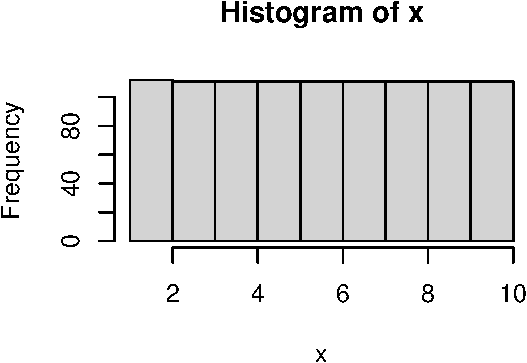
\includegraphics{homework6_files/figure-latex/unnamed-chunk-10-1.pdf}

\hypertarget{b-fit-the-regression-of-observed-on-snowdepth-wind-tempf-cloud-grpsize-voc-and-suco.-test-the-significance-of-cloud-cover-in-this-model.}{%
\subsubsection{(3b) Fit the regression of observed on snowdepth, wind,
tempf, cloud, grpsize, voc, and suco. Test the significance of cloud
cover in this
model.}\label{b-fit-the-regression-of-observed-on-snowdepth-wind-tempf-cloud-grpsize-voc-and-suco.-test-the-significance-of-cloud-cover-in-this-model.}}

\begin{Shaded}
\begin{Highlighting}[]
\NormalTok{sight\_logit }\OtherTok{\textless{}{-}} \FunctionTok{glm}\NormalTok{(observed }\SpecialCharTok{\textasciitilde{}}\NormalTok{ snowdepth }\SpecialCharTok{+}\NormalTok{ wind }\SpecialCharTok{+}\NormalTok{ tempf }\SpecialCharTok{+}\NormalTok{ cloud }\SpecialCharTok{+}\NormalTok{ grpsize }\SpecialCharTok{+}\NormalTok{ voc }\SpecialCharTok{+}\NormalTok{ suco, }\AttributeTok{family =}\NormalTok{ binomial, }\AttributeTok{data =}\NormalTok{ sight)}
\FunctionTok{summary}\NormalTok{(sight\_logit)}

\NormalTok{Call}\SpecialCharTok{:}
\FunctionTok{glm}\NormalTok{(}\AttributeTok{formula =}\NormalTok{ observed }\SpecialCharTok{\textasciitilde{}}\NormalTok{ snowdepth }\SpecialCharTok{+}\NormalTok{ wind }\SpecialCharTok{+}\NormalTok{ tempf }\SpecialCharTok{+}\NormalTok{ cloud }\SpecialCharTok{+}\NormalTok{ grpsize }\SpecialCharTok{+} 
\NormalTok{    voc }\SpecialCharTok{+}\NormalTok{ suco, }\AttributeTok{family =}\NormalTok{ binomial, }\AttributeTok{data =}\NormalTok{ sight)}

\NormalTok{Deviance Residuals}\SpecialCharTok{:} 
\NormalTok{    Min       1Q   Median       3Q      Max  }
\SpecialCharTok{{-}}\FloatTok{1.9777}  \SpecialCharTok{{-}}\FloatTok{0.8395}  \SpecialCharTok{{-}}\FloatTok{0.4563}   \FloatTok{1.0106}   \FloatTok{1.9756}  

\NormalTok{Coefficients}\SpecialCharTok{:}
\NormalTok{                   Estimate Std. Error z value }\FunctionTok{Pr}\NormalTok{(}\SpecialCharTok{\textgreater{}}\ErrorTok{|}\NormalTok{z}\SpecialCharTok{|}\NormalTok{)    }
\NormalTok{(Intercept)        }\FloatTok{1.310467}   \FloatTok{1.403007}   \FloatTok{0.934}    \FloatTok{0.350}    
\NormalTok{snowdepth}\SpecialCharTok{\textgreater{}}\NormalTok{16in     }\FloatTok{0.848727}   \FloatTok{0.934197}   \FloatTok{0.909}    \FloatTok{0.364}    
\NormalTok{snowdepth8}\SpecialCharTok{{-}}\NormalTok{16in    }\FloatTok{0.409133}   \FloatTok{0.841835}   \FloatTok{0.486}    \FloatTok{0.627}    
\NormalTok{wind              }\SpecialCharTok{{-}}\FloatTok{0.020232}   \FloatTok{0.071242}  \SpecialCharTok{{-}}\FloatTok{0.284}    \FloatTok{0.776}    
\NormalTok{tempf             }\SpecialCharTok{{-}}\FloatTok{0.018944}   \FloatTok{0.025973}  \SpecialCharTok{{-}}\FloatTok{0.729}    \FloatTok{0.466}    
\NormalTok{cloud1}\DecValTok{{-}25}\NormalTok{\%        }\SpecialCharTok{{-}}\FloatTok{0.947854}   \FloatTok{0.687524}  \SpecialCharTok{{-}}\FloatTok{1.379}    \FloatTok{0.168}    
\NormalTok{cloud26}\DecValTok{{-}50}\NormalTok{\%       }\SpecialCharTok{{-}}\FloatTok{0.646409}   \FloatTok{1.007295}  \SpecialCharTok{{-}}\FloatTok{0.642}    \FloatTok{0.521}    
\NormalTok{cloud51}\DecValTok{{-}75}\NormalTok{\%       }\SpecialCharTok{{-}}\FloatTok{0.010123}   \FloatTok{1.049082}  \SpecialCharTok{{-}}\FloatTok{0.010}    \FloatTok{0.992}    
\NormalTok{cloud76}\DecValTok{{-}100}\NormalTok{\%       }\FloatTok{0.046656}   \FloatTok{0.609258}   \FloatTok{0.077}    \FloatTok{0.939}    
\NormalTok{grpsize            }\FloatTok{0.296209}   \FloatTok{0.242907}   \FloatTok{1.219}    \FloatTok{0.223}    
\NormalTok{voc               }\SpecialCharTok{{-}}\FloatTok{0.036234}   \FloatTok{0.008593}  \SpecialCharTok{{-}}\FloatTok{4.217} \FloatTok{2.48e{-}05} \SpecialCharTok{**}\ErrorTok{*}
\NormalTok{sucomarginal}\SpecialCharTok{/}\NormalTok{poor }\SpecialCharTok{{-}}\FloatTok{0.230966}   \FloatTok{0.773954}  \SpecialCharTok{{-}}\FloatTok{0.298}    \FloatTok{0.765}    
\SpecialCharTok{{-}{-}{-}}
\NormalTok{Signif. codes}\SpecialCharTok{:}  \DecValTok{0} \StringTok{\textquotesingle{}***\textquotesingle{}} \FloatTok{0.001} \StringTok{\textquotesingle{}**\textquotesingle{}} \FloatTok{0.01} \StringTok{\textquotesingle{}*\textquotesingle{}} \FloatTok{0.05} \StringTok{\textquotesingle{}.\textquotesingle{}} \FloatTok{0.1} \StringTok{\textquotesingle{} \textquotesingle{}} \DecValTok{1}

\NormalTok{(Dispersion parameter }\ControlFlowTok{for}\NormalTok{ binomial family taken to be }\DecValTok{1}\NormalTok{)}

\NormalTok{    Null deviance}\SpecialCharTok{:} \FloatTok{171.61}\NormalTok{  on }\DecValTok{123}\NormalTok{  degrees of freedom}
\NormalTok{Residual deviance}\SpecialCharTok{:} \FloatTok{136.69}\NormalTok{  on }\DecValTok{112}\NormalTok{  degrees of freedom}
\NormalTok{AIC}\SpecialCharTok{:} \FloatTok{160.69}

\NormalTok{Number of Fisher Scoring iterations}\SpecialCharTok{:} \DecValTok{4}
\end{Highlighting}
\end{Shaded}

\hypertarget{c-starting-with-your-part-b-model-use-backwards-selection-to-find-the-most-significant-predictors-of-sightability.-you-do-not-need-to-check-for-assumptions-or-outliers.-the-assumptions-seem-to-be-met-and-there-are-no-unusually-influential-cases.-you-do-need-to-give-a-step-by-step-description-of-your-model-selection-including-hypotheses-and-p-values-given-at-each-step-to-justify-the-elimination-of-each-variable-you-throw-out.}{%
\subsubsection{\texorpdfstring{(3c) Starting with your part (b) model,
use backwards selection to find the most significant predictors of
sightability. You \textbf{do not(!)} need to check for assumptions or
outliers. (The assumptions seem to be met and there are no unusually
influential cases.) You \textbf{do} need to give a step-by-step
description of your model selection, including hypotheses and p-values
given at each step to justify the elimination of each variable you throw
out.}{(3c) Starting with your part (b) model, use backwards selection to find the most significant predictors of sightability. You do not(!) need to check for assumptions or outliers. (The assumptions seem to be met and there are no unusually influential cases.) You do need to give a step-by-step description of your model selection, including hypotheses and p-values given at each step to justify the elimination of each variable you throw out.}}\label{c-starting-with-your-part-b-model-use-backwards-selection-to-find-the-most-significant-predictors-of-sightability.-you-do-not-need-to-check-for-assumptions-or-outliers.-the-assumptions-seem-to-be-met-and-there-are-no-unusually-influential-cases.-you-do-need-to-give-a-step-by-step-description-of-your-model-selection-including-hypotheses-and-p-values-given-at-each-step-to-justify-the-elimination-of-each-variable-you-throw-out.}}

\begin{Shaded}
\begin{Highlighting}[]
\NormalTok{new1\_glm }\OtherTok{\textless{}{-}} \FunctionTok{glm}\NormalTok{(observed }\SpecialCharTok{\textasciitilde{}}\NormalTok{ snowdepth }\SpecialCharTok{+}\NormalTok{ wind }\SpecialCharTok{+}\NormalTok{ tempf }\SpecialCharTok{+}\NormalTok{ cloud }\SpecialCharTok{+}\NormalTok{ grpsize }\SpecialCharTok{+}\NormalTok{ voc, }\AttributeTok{family =}\NormalTok{ binomial, }\AttributeTok{data =}\NormalTok{ sight)}
\NormalTok{new2\_glm }\OtherTok{\textless{}{-}} \FunctionTok{glm}\NormalTok{(observed }\SpecialCharTok{\textasciitilde{}}\NormalTok{ snowdepth }\SpecialCharTok{+}\NormalTok{ wind }\SpecialCharTok{+}\NormalTok{ tempf }\SpecialCharTok{+}\NormalTok{ cloud }\SpecialCharTok{+}\NormalTok{ grpsize, }\AttributeTok{family =}\NormalTok{ binomial, }\AttributeTok{data =}\NormalTok{ sight)}
\NormalTok{new3\_glm }\OtherTok{\textless{}{-}} \FunctionTok{glm}\NormalTok{(observed }\SpecialCharTok{\textasciitilde{}}\NormalTok{ snowdepth }\SpecialCharTok{+}\NormalTok{ wind }\SpecialCharTok{+}\NormalTok{ tempf }\SpecialCharTok{+}\NormalTok{ cloud, }\AttributeTok{family =}\NormalTok{ binomial, }\AttributeTok{data =}\NormalTok{ sight)}
\NormalTok{new4\_glm }\OtherTok{\textless{}{-}} \FunctionTok{glm}\NormalTok{(observed }\SpecialCharTok{\textasciitilde{}}\NormalTok{ snowdepth }\SpecialCharTok{+}\NormalTok{ wind }\SpecialCharTok{+}\NormalTok{ tempf, }\AttributeTok{family =}\NormalTok{ binomial, }\AttributeTok{data =}\NormalTok{ sight)}
\NormalTok{new5\_glm }\OtherTok{\textless{}{-}} \FunctionTok{glm}\NormalTok{(observed }\SpecialCharTok{\textasciitilde{}}\NormalTok{ snowdepth }\SpecialCharTok{+}\NormalTok{ wind, }\AttributeTok{family =}\NormalTok{ binomial, }\AttributeTok{data =}\NormalTok{ sight)}
\NormalTok{new6\_glm }\OtherTok{\textless{}{-}} \FunctionTok{glm}\NormalTok{(observed }\SpecialCharTok{\textasciitilde{}}\NormalTok{ snowdepth, }\AttributeTok{family =}\NormalTok{ binomial, }\AttributeTok{data =}\NormalTok{ sight)}
\FunctionTok{anova}\NormalTok{(new1\_glm, sight\_logit, }\AttributeTok{test=}\StringTok{"Chisq"}\NormalTok{)}
\NormalTok{Analysis of Deviance Table}

\NormalTok{Model }\DecValTok{1}\SpecialCharTok{:}\NormalTok{ observed }\SpecialCharTok{\textasciitilde{}}\NormalTok{ snowdepth }\SpecialCharTok{+}\NormalTok{ wind }\SpecialCharTok{+}\NormalTok{ tempf }\SpecialCharTok{+}\NormalTok{ cloud }\SpecialCharTok{+}\NormalTok{ grpsize }\SpecialCharTok{+}\NormalTok{ voc}
\NormalTok{Model }\DecValTok{2}\SpecialCharTok{:}\NormalTok{ observed }\SpecialCharTok{\textasciitilde{}}\NormalTok{ snowdepth }\SpecialCharTok{+}\NormalTok{ wind }\SpecialCharTok{+}\NormalTok{ tempf }\SpecialCharTok{+}\NormalTok{ cloud }\SpecialCharTok{+}\NormalTok{ grpsize }\SpecialCharTok{+}\NormalTok{ voc }\SpecialCharTok{+} 
\NormalTok{    suco}
\NormalTok{  Resid. Df Resid. Dev Df Deviance }\FunctionTok{Pr}\NormalTok{(}\SpecialCharTok{\textgreater{}}\NormalTok{Chi)}
\DecValTok{1}       \DecValTok{113}     \FloatTok{136.78}                     
\DecValTok{2}       \DecValTok{112}     \FloatTok{136.69}  \DecValTok{1} \FloatTok{0.088993}   \FloatTok{0.7655}
\FunctionTok{anova}\NormalTok{(new2\_glm, sight\_logit, }\AttributeTok{test=}\StringTok{"Chisq"}\NormalTok{)}
\NormalTok{Analysis of Deviance Table}

\NormalTok{Model }\DecValTok{1}\SpecialCharTok{:}\NormalTok{ observed }\SpecialCharTok{\textasciitilde{}}\NormalTok{ snowdepth }\SpecialCharTok{+}\NormalTok{ wind }\SpecialCharTok{+}\NormalTok{ tempf }\SpecialCharTok{+}\NormalTok{ cloud }\SpecialCharTok{+}\NormalTok{ grpsize}
\NormalTok{Model }\DecValTok{2}\SpecialCharTok{:}\NormalTok{ observed }\SpecialCharTok{\textasciitilde{}}\NormalTok{ snowdepth }\SpecialCharTok{+}\NormalTok{ wind }\SpecialCharTok{+}\NormalTok{ tempf }\SpecialCharTok{+}\NormalTok{ cloud }\SpecialCharTok{+}\NormalTok{ grpsize }\SpecialCharTok{+}\NormalTok{ voc }\SpecialCharTok{+} 
\NormalTok{    suco}
\NormalTok{  Resid. Df Resid. Dev Df Deviance  }\FunctionTok{Pr}\NormalTok{(}\SpecialCharTok{\textgreater{}}\NormalTok{Chi)    }
\DecValTok{1}       \DecValTok{114}     \FloatTok{158.13}                          
\DecValTok{2}       \DecValTok{112}     \FloatTok{136.69}  \DecValTok{2}   \FloatTok{21.439} \FloatTok{2.211e{-}05} \SpecialCharTok{**}\ErrorTok{*}
\SpecialCharTok{{-}{-}{-}}
\NormalTok{Signif. codes}\SpecialCharTok{:}  \DecValTok{0} \StringTok{\textquotesingle{}***\textquotesingle{}} \FloatTok{0.001} \StringTok{\textquotesingle{}**\textquotesingle{}} \FloatTok{0.01} \StringTok{\textquotesingle{}*\textquotesingle{}} \FloatTok{0.05} \StringTok{\textquotesingle{}.\textquotesingle{}} \FloatTok{0.1} \StringTok{\textquotesingle{} \textquotesingle{}} \DecValTok{1}
\FunctionTok{anova}\NormalTok{(new3\_glm, sight\_logit, }\AttributeTok{test=}\StringTok{"Chisq"}\NormalTok{)}
\NormalTok{Analysis of Deviance Table}

\NormalTok{Model }\DecValTok{1}\SpecialCharTok{:}\NormalTok{ observed }\SpecialCharTok{\textasciitilde{}}\NormalTok{ snowdepth }\SpecialCharTok{+}\NormalTok{ wind }\SpecialCharTok{+}\NormalTok{ tempf }\SpecialCharTok{+}\NormalTok{ cloud}
\NormalTok{Model }\DecValTok{2}\SpecialCharTok{:}\NormalTok{ observed }\SpecialCharTok{\textasciitilde{}}\NormalTok{ snowdepth }\SpecialCharTok{+}\NormalTok{ wind }\SpecialCharTok{+}\NormalTok{ tempf }\SpecialCharTok{+}\NormalTok{ cloud }\SpecialCharTok{+}\NormalTok{ grpsize }\SpecialCharTok{+}\NormalTok{ voc }\SpecialCharTok{+} 
\NormalTok{    suco}
\NormalTok{  Resid. Df Resid. Dev Df Deviance }\FunctionTok{Pr}\NormalTok{(}\SpecialCharTok{\textgreater{}}\NormalTok{Chi)    }
\DecValTok{1}       \DecValTok{115}     \FloatTok{162.39}                         
\DecValTok{2}       \DecValTok{112}     \FloatTok{136.69}  \DecValTok{3}   \FloatTok{25.704}  \FloatTok{1.1e{-}05} \SpecialCharTok{**}\ErrorTok{*}
\SpecialCharTok{{-}{-}{-}}
\NormalTok{Signif. codes}\SpecialCharTok{:}  \DecValTok{0} \StringTok{\textquotesingle{}***\textquotesingle{}} \FloatTok{0.001} \StringTok{\textquotesingle{}**\textquotesingle{}} \FloatTok{0.01} \StringTok{\textquotesingle{}*\textquotesingle{}} \FloatTok{0.05} \StringTok{\textquotesingle{}.\textquotesingle{}} \FloatTok{0.1} \StringTok{\textquotesingle{} \textquotesingle{}} \DecValTok{1}
\FunctionTok{anova}\NormalTok{(new4\_glm, sight\_logit, }\AttributeTok{test=}\StringTok{"Chisq"}\NormalTok{)}
\NormalTok{Analysis of Deviance Table}

\NormalTok{Model }\DecValTok{1}\SpecialCharTok{:}\NormalTok{ observed }\SpecialCharTok{\textasciitilde{}}\NormalTok{ snowdepth }\SpecialCharTok{+}\NormalTok{ wind }\SpecialCharTok{+}\NormalTok{ tempf}
\NormalTok{Model }\DecValTok{2}\SpecialCharTok{:}\NormalTok{ observed }\SpecialCharTok{\textasciitilde{}}\NormalTok{ snowdepth }\SpecialCharTok{+}\NormalTok{ wind }\SpecialCharTok{+}\NormalTok{ tempf }\SpecialCharTok{+}\NormalTok{ cloud }\SpecialCharTok{+}\NormalTok{ grpsize }\SpecialCharTok{+}\NormalTok{ voc }\SpecialCharTok{+} 
\NormalTok{    suco}
\NormalTok{  Resid. Df Resid. Dev Df Deviance  }\FunctionTok{Pr}\NormalTok{(}\SpecialCharTok{\textgreater{}}\NormalTok{Chi)    }
\DecValTok{1}       \DecValTok{119}     \FloatTok{165.35}                          
\DecValTok{2}       \DecValTok{112}     \FloatTok{136.69}  \DecValTok{7}   \FloatTok{28.666} \FloatTok{0.0001665} \SpecialCharTok{**}\ErrorTok{*}
\SpecialCharTok{{-}{-}{-}}
\NormalTok{Signif. codes}\SpecialCharTok{:}  \DecValTok{0} \StringTok{\textquotesingle{}***\textquotesingle{}} \FloatTok{0.001} \StringTok{\textquotesingle{}**\textquotesingle{}} \FloatTok{0.01} \StringTok{\textquotesingle{}*\textquotesingle{}} \FloatTok{0.05} \StringTok{\textquotesingle{}.\textquotesingle{}} \FloatTok{0.1} \StringTok{\textquotesingle{} \textquotesingle{}} \DecValTok{1}
\FunctionTok{anova}\NormalTok{(new5\_glm, sight\_logit, }\AttributeTok{test=}\StringTok{"Chisq"}\NormalTok{)}
\NormalTok{Analysis of Deviance Table}

\NormalTok{Model }\DecValTok{1}\SpecialCharTok{:}\NormalTok{ observed }\SpecialCharTok{\textasciitilde{}}\NormalTok{ snowdepth }\SpecialCharTok{+}\NormalTok{ wind}
\NormalTok{Model }\DecValTok{2}\SpecialCharTok{:}\NormalTok{ observed }\SpecialCharTok{\textasciitilde{}}\NormalTok{ snowdepth }\SpecialCharTok{+}\NormalTok{ wind }\SpecialCharTok{+}\NormalTok{ tempf }\SpecialCharTok{+}\NormalTok{ cloud }\SpecialCharTok{+}\NormalTok{ grpsize }\SpecialCharTok{+}\NormalTok{ voc }\SpecialCharTok{+} 
\NormalTok{    suco}
\NormalTok{  Resid. Df Resid. Dev Df Deviance  }\FunctionTok{Pr}\NormalTok{(}\SpecialCharTok{\textgreater{}}\NormalTok{Chi)    }
\DecValTok{1}       \DecValTok{120}     \FloatTok{166.27}                          
\DecValTok{2}       \DecValTok{112}     \FloatTok{136.69}  \DecValTok{8}    \FloatTok{29.58} \FloatTok{0.0002508} \SpecialCharTok{**}\ErrorTok{*}
\SpecialCharTok{{-}{-}{-}}
\NormalTok{Signif. codes}\SpecialCharTok{:}  \DecValTok{0} \StringTok{\textquotesingle{}***\textquotesingle{}} \FloatTok{0.001} \StringTok{\textquotesingle{}**\textquotesingle{}} \FloatTok{0.01} \StringTok{\textquotesingle{}*\textquotesingle{}} \FloatTok{0.05} \StringTok{\textquotesingle{}.\textquotesingle{}} \FloatTok{0.1} \StringTok{\textquotesingle{} \textquotesingle{}} \DecValTok{1}
\FunctionTok{anova}\NormalTok{(new6\_glm, sight\_logit, }\AttributeTok{test=}\StringTok{"Chisq"}\NormalTok{)}
\NormalTok{Analysis of Deviance Table}

\NormalTok{Model }\DecValTok{1}\SpecialCharTok{:}\NormalTok{ observed }\SpecialCharTok{\textasciitilde{}}\NormalTok{ snowdepth}
\NormalTok{Model }\DecValTok{2}\SpecialCharTok{:}\NormalTok{ observed }\SpecialCharTok{\textasciitilde{}}\NormalTok{ snowdepth }\SpecialCharTok{+}\NormalTok{ wind }\SpecialCharTok{+}\NormalTok{ tempf }\SpecialCharTok{+}\NormalTok{ cloud }\SpecialCharTok{+}\NormalTok{ grpsize }\SpecialCharTok{+}\NormalTok{ voc }\SpecialCharTok{+} 
\NormalTok{    suco}
\NormalTok{  Resid. Df Resid. Dev Df Deviance  }\FunctionTok{Pr}\NormalTok{(}\SpecialCharTok{\textgreater{}}\NormalTok{Chi)    }
\DecValTok{1}       \DecValTok{121}     \FloatTok{167.10}                          
\DecValTok{2}       \DecValTok{112}     \FloatTok{136.69}  \DecValTok{9}    \FloatTok{30.41} \FloatTok{0.0003735} \SpecialCharTok{**}\ErrorTok{*}
\SpecialCharTok{{-}{-}{-}}
\NormalTok{Signif. codes}\SpecialCharTok{:}  \DecValTok{0} \StringTok{\textquotesingle{}***\textquotesingle{}} \FloatTok{0.001} \StringTok{\textquotesingle{}**\textquotesingle{}} \FloatTok{0.01} \StringTok{\textquotesingle{}*\textquotesingle{}} \FloatTok{0.05} \StringTok{\textquotesingle{}.\textquotesingle{}} \FloatTok{0.1} \StringTok{\textquotesingle{} \textquotesingle{}} \DecValTok{1}
\end{Highlighting}
\end{Shaded}

Looking at the p-values for each backward selection step, we see that we
can drop everything but the voc variable, only voc has a significant
p-value (p = 2.48e-05)

\hypertarget{d-the-mn-dnr-concluded-that-voc-is-the-most-important-predictor-of-sightability-if-your-results-for-part-c-disagree-you-may-want-to-redo-your-model-selection.-use-your-best-model-from-part-c-to-determine-how-increasing-voc-by-5-percentage-points-will-effect-the-odds-of-sighting-a-moose.-also-give-a-95-confidence-interval-for-this-effect.}{%
\subsubsection{(3d) The MN DNR concluded that voc is the most important
predictor of sightability (if your results for part (c) disagree, you
may want to redo your model selection!). Use your ``best" model from
part (c) to determine how increasing voc by 5 percentage points will
effect the odds of sighting a moose. Also give a 95\% confidence
interval for this
effect.}\label{d-the-mn-dnr-concluded-that-voc-is-the-most-important-predictor-of-sightability-if-your-results-for-part-c-disagree-you-may-want-to-redo-your-model-selection.-use-your-best-model-from-part-c-to-determine-how-increasing-voc-by-5-percentage-points-will-effect-the-odds-of-sighting-a-moose.-also-give-a-95-confidence-interval-for-this-effect.}}

\begin{Shaded}
\begin{Highlighting}[]
\FunctionTok{summary}\NormalTok{(new6\_glm)}

\NormalTok{Call}\SpecialCharTok{:}
\FunctionTok{glm}\NormalTok{(}\AttributeTok{formula =}\NormalTok{ observed }\SpecialCharTok{\textasciitilde{}}\NormalTok{ snowdepth, }\AttributeTok{family =}\NormalTok{ binomial, }\AttributeTok{data =}\NormalTok{ sight)}

\NormalTok{Deviance Residuals}\SpecialCharTok{:} 
\NormalTok{    Min       1Q   Median       3Q      Max  }
\SpecialCharTok{{-}}\FloatTok{1.2453}  \SpecialCharTok{{-}}\FloatTok{1.2453}  \SpecialCharTok{{-}}\FloatTok{0.8842}   \FloatTok{1.1110}   \FloatTok{1.5023}  

\NormalTok{Coefficients}\SpecialCharTok{:}
\NormalTok{                Estimate Std. Error z value }\FunctionTok{Pr}\NormalTok{(}\SpecialCharTok{\textgreater{}}\ErrorTok{|}\NormalTok{z}\SpecialCharTok{|}\NormalTok{)  }
\NormalTok{(Intercept)      }\SpecialCharTok{{-}}\FloatTok{0.7376}     \FloatTok{0.3666}  \SpecialCharTok{{-}}\FloatTok{2.012}   \FloatTok{0.0442} \SpecialCharTok{*}
\NormalTok{snowdepth}\SpecialCharTok{\textgreater{}}\NormalTok{16in    }\FloatTok{0.8958}     \FloatTok{0.4328}   \FloatTok{2.070}   \FloatTok{0.0385} \SpecialCharTok{*}
\NormalTok{snowdepth8}\SpecialCharTok{{-}}\NormalTok{16in   }\FloatTok{0.7376}     \FloatTok{0.6482}   \FloatTok{1.138}   \FloatTok{0.2551}  
\SpecialCharTok{{-}{-}{-}}
\NormalTok{Signif. codes}\SpecialCharTok{:}  \DecValTok{0} \StringTok{\textquotesingle{}***\textquotesingle{}} \FloatTok{0.001} \StringTok{\textquotesingle{}**\textquotesingle{}} \FloatTok{0.01} \StringTok{\textquotesingle{}*\textquotesingle{}} \FloatTok{0.05} \StringTok{\textquotesingle{}.\textquotesingle{}} \FloatTok{0.1} \StringTok{\textquotesingle{} \textquotesingle{}} \DecValTok{1}

\NormalTok{(Dispersion parameter }\ControlFlowTok{for}\NormalTok{ binomial family taken to be }\DecValTok{1}\NormalTok{)}

\NormalTok{    Null deviance}\SpecialCharTok{:} \FloatTok{171.61}\NormalTok{  on }\DecValTok{123}\NormalTok{  degrees of freedom}
\NormalTok{Residual deviance}\SpecialCharTok{:} \FloatTok{167.10}\NormalTok{  on }\DecValTok{121}\NormalTok{  degrees of freedom}
\NormalTok{AIC}\SpecialCharTok{:} \FloatTok{173.1}

\NormalTok{Number of Fisher Scoring iterations}\SpecialCharTok{:} \DecValTok{4}
\FunctionTok{confint}\NormalTok{(new6\_glm)}
                      \FloatTok{2.5} \SpecialCharTok{\%      97.5 \%}
\NormalTok{(Intercept)     }\SpecialCharTok{{-}}\FloatTok{1.49494441} \SpecialCharTok{{-}}\FloatTok{0.04178323}
\NormalTok{snowdepth}\SpecialCharTok{\textgreater{}}\NormalTok{16in   }\FloatTok{0.06484944}  \FloatTok{1.77276804}
\NormalTok{snowdepth8}\SpecialCharTok{{-}}\NormalTok{16in }\SpecialCharTok{{-}}\FloatTok{0.53899501}  \FloatTok{2.03275439}
\FunctionTok{exp}\NormalTok{(}\SpecialCharTok{{-}}\FloatTok{0.05082098} \SpecialCharTok{*} \DecValTok{5}\NormalTok{)}
\NormalTok{[}\DecValTok{1}\NormalTok{] }\FloatTok{0.7756104}
\FunctionTok{exp}\NormalTok{(}\SpecialCharTok{{-}}\FloatTok{0.02025314} \SpecialCharTok{*} \DecValTok{5}\NormalTok{)}
\NormalTok{[}\DecValTok{1}\NormalTok{] }\FloatTok{0.9036929}
\end{Highlighting}
\end{Shaded}

\hypertarget{looking-at-the-calculations-above-we-see-that-a-5-percent-increase-in-voc-results-in-a-0.840331-multiplicative-change-in-the-odds.-thus-decreasing-odds-by-approx.-16.-we-are-95-confident-that-a-5-percent-change-in-moose-sighting-odds-would-be-a-factor-between-the-values-of-0.7756104-0.9036929.}{%
\subsection{Looking at the calculations above, we see that a 5 percent
increase in voc results in a 0.840331 multiplicative change in the odds.
Thus, decreasing odds by approx. 16\%. We are 95\% confident that a 5
percent change in moose sighting odds would be a factor between the
values of 0.7756104,
0.9036929.}\label{looking-at-the-calculations-above-we-see-that-a-5-percent-increase-in-voc-results-in-a-0.840331-multiplicative-change-in-the-odds.-thus-decreasing-odds-by-approx.-16.-we-are-95-confident-that-a-5-percent-change-in-moose-sighting-odds-would-be-a-factor-between-the-values-of-0.7756104-0.9036929.}}

\hypertarget{problem-4-tire-failure-on-ford-explorers-ch.-20-exercise-18}{%
\subsection{Problem 4: Tire failure on Ford Explorers (ch.~20 exercise
18)}\label{problem-4-tire-failure-on-ford-explorers-ch.-20-exercise-18}}

Read the data set description for exercise 18, then use the data
provided (\texttt{ex2018}) to answer the following questions.

\hypertarget{a-the-textbook-also-suggests-an-interaction-between-vehicle-type-make-and-number-of-passengers.-to-explore-this-interaction-create-a-side-by-side-boxplot-of-passengers-by-cause-that-is-faceted-by-make.-carefully-explain-why-this-graph-suggests-that-we-should-add-the-interaction-between-vehicle-type-and-number-of-passengers-in-the-model-for-odds-of-tire-failure.}{%
\subsubsection{\texorpdfstring{(4a) The textbook also suggests an
interaction between vehicle type (\texttt{Make}) and number of
\texttt{Passengers}. To explore this interaction, create a side-by-side
boxplot of \texttt{Passengers} by \texttt{Cause} that is faceted by
\texttt{Make}. Carefully explain why this graph suggests that we should
add the interaction between vehicle type and number of Passengers in the
model for odds of tire
failure.}{(4a) The textbook also suggests an interaction between vehicle type (Make) and number of Passengers. To explore this interaction, create a side-by-side boxplot of Passengers by Cause that is faceted by Make. Carefully explain why this graph suggests that we should add the interaction between vehicle type and number of Passengers in the model for odds of tire failure.}}\label{a-the-textbook-also-suggests-an-interaction-between-vehicle-type-make-and-number-of-passengers.-to-explore-this-interaction-create-a-side-by-side-boxplot-of-passengers-by-cause-that-is-faceted-by-make.-carefully-explain-why-this-graph-suggests-that-we-should-add-the-interaction-between-vehicle-type-and-number-of-passengers-in-the-model-for-odds-of-tire-failure.}}

\begin{Shaded}
\begin{Highlighting}[]
\NormalTok{ex2018 }\OtherTok{=}\NormalTok{ ex2018}
\FunctionTok{library}\NormalTok{(ggplot2)}
\FunctionTok{ggplot}\NormalTok{(ex2018, }\FunctionTok{aes}\NormalTok{(}\AttributeTok{x =}\NormalTok{ Passengers, }\AttributeTok{y =}\NormalTok{ Cause)) }\SpecialCharTok{+}
 \FunctionTok{geom\_boxplot}\NormalTok{() }\SpecialCharTok{+}
\FunctionTok{facet\_wrap}\NormalTok{(}\SpecialCharTok{\textasciitilde{}}\NormalTok{Make)}
\end{Highlighting}
\end{Shaded}

\includegraphics{homework6_files/figure-latex/unnamed-chunk-14-1.pdf}
Looking at the pair of boxplots above, we can clearly see that there is
a difference between the average tire failure passenger count for Ford
and other cars with the average Ford tire failure passenger count being
approx. 3 passengers and the average other model tire failure passenger
count being approx. less than 1 passenger (there is a larger gap between
passenger count of with-tire and without-tire failure for Ford and other
models). This would be explained by the existence of and interactive
effect between vehicle type and passenger.

\hypertarget{b-fit-the-logistic-regression-of-cause-on-age-age2-number-of-passengers-vehicle-make-and-the-interaction-of-passengers-and-make.-write-down-the-fitted-equation-for-fords-and-non-ford-vehicles.}{%
\subsubsection{\texorpdfstring{(4b) Fit the logistic regression of cause
on age, age\(^2\), number of passengers, vehicle make, and the
interaction of passengers and make. Write down the fitted equation for
Fords and non-Ford
vehicles.}{(4b) Fit the logistic regression of cause on age, age\^{}2, number of passengers, vehicle make, and the interaction of passengers and make. Write down the fitted equation for Fords and non-Ford vehicles.}}\label{b-fit-the-logistic-regression-of-cause-on-age-age2-number-of-passengers-vehicle-make-and-the-interaction-of-passengers-and-make.-write-down-the-fitted-equation-for-fords-and-non-ford-vehicles.}}

\begin{Shaded}
\begin{Highlighting}[]
\NormalTok{ex2018\_glm }\OtherTok{\textless{}{-}} \FunctionTok{glm}\NormalTok{(Cause }\SpecialCharTok{\textasciitilde{}}\NormalTok{ VehicleAge }\SpecialCharTok{+} \FunctionTok{I}\NormalTok{(VehicleAge}\SpecialCharTok{\^{}}\DecValTok{2}\NormalTok{) }\SpecialCharTok{+}\NormalTok{ Passengers}\SpecialCharTok{*}\NormalTok{Make, }\AttributeTok{family =}\NormalTok{ binomial, }\AttributeTok{data =}\NormalTok{ ex2018)}
\FunctionTok{tidy}\NormalTok{(ex2018\_glm)}
\CommentTok{\# A tibble: 6 x 5}
\NormalTok{  term                 estimate std.error statistic      p.value}
  \SpecialCharTok{\textless{}}\NormalTok{chr}\SpecialCharTok{\textgreater{}}                   \ErrorTok{\textless{}}\NormalTok{dbl}\SpecialCharTok{\textgreater{}}     \ErrorTok{\textless{}}\NormalTok{dbl}\SpecialCharTok{\textgreater{}}     \ErrorTok{\textless{}}\NormalTok{dbl}\SpecialCharTok{\textgreater{}}        \ErrorTok{\textless{}}\NormalTok{dbl}\SpecialCharTok{\textgreater{}}
\DecValTok{1}\NormalTok{ (Intercept)           }\SpecialCharTok{{-}}\FloatTok{10.8}       \FloatTok{2.23}      \SpecialCharTok{{-}}\FloatTok{4.87} \FloatTok{0.00000110}  
\DecValTok{2}\NormalTok{ VehicleAge              }\FloatTok{3.42}      \FloatTok{1.30}       \FloatTok{2.62} \FloatTok{0.00871}     
\DecValTok{3} \FunctionTok{I}\NormalTok{(VehicleAge}\SpecialCharTok{\^{}}\DecValTok{2}\NormalTok{)        }\SpecialCharTok{{-}}\FloatTok{0.396}     \FloatTok{0.194}     \SpecialCharTok{{-}}\FloatTok{2.04} \FloatTok{0.0412}      
\DecValTok{4}\NormalTok{ Passengers              }\FloatTok{0.839}     \FloatTok{0.149}      \FloatTok{5.65} \FloatTok{0.0000000159}
\DecValTok{5}\NormalTok{ MakeOther              }\SpecialCharTok{{-}}\FloatTok{1.53}      \FloatTok{0.717}     \SpecialCharTok{{-}}\FloatTok{2.14} \FloatTok{0.0326}      
\DecValTok{6}\NormalTok{ Passengers}\SpecialCharTok{:}\NormalTok{MakeOther   }\SpecialCharTok{{-}}\FloatTok{0.636}     \FloatTok{0.330}     \SpecialCharTok{{-}}\FloatTok{1.93} \FloatTok{0.0539}      
\end{Highlighting}
\end{Shaded}

\(logit(Tire) = -10.8474912 + 3.4211526(VehicleAge) - 0.3961082(VehicleAge^2) + 0.8393122(Passengers)\)
\newline
\(logit(Tire) = -10.8474912 + 3.4211526(VehicleAge) - 0.3961082(VehicleAge^2) + 0.8393122(Passengers) - 1.5321682(MakeOther) - 0.6359625(Passengers)(MakeOther)\)

\hypertarget{c-what-is-the-effect-of-vehicle-type-on-the-odds-of-tire-failure-give-your-answer-as-an-odds-ratio-formula-involving-model-cofficient-estimates-and-the-variable-passengers.-clearly-state-what-the-odds-ratio-is-measuring-odds-of-for-group-vs.-.-note-this-answer-will-be-an-equation-involving-passengers.-you-will-get-actual-odds-ration-numbers-in-part-d.}{%
\subsubsection{(4c) What is the effect of vehicle type on the odds of
tire failure? Give your answer as an odds ratio formula involving model
cofficient estimates and the variable passengers. Clearly state what the
odds ratio is measuring (odds of ? for group ? vs.~?). (Note: this
answer will be an equation involving passengers. You will get actual
odds ration numbers in part
d.)}\label{c-what-is-the-effect-of-vehicle-type-on-the-odds-of-tire-failure-give-your-answer-as-an-odds-ratio-formula-involving-model-cofficient-estimates-and-the-variable-passengers.-clearly-state-what-the-odds-ratio-is-measuring-odds-of-for-group-vs.-.-note-this-answer-will-be-an-equation-involving-passengers.-you-will-get-actual-odds-ration-numbers-in-part-d.}}

\(odds = \frac{e^{-10.8474912 + 3.4211526(VehicleAge) - 0.3961082(VehicleAge^2) + 0.8393122(Passengers)}}{e^{-10.8474912 + 3.4211526(VehicleAge) - 0.3961082(VehicleAge^2) + 0.8393122(Passengers) - 1.5321682(MakeOther) - 0.6359625(Passengers)(MakeOther)}}\)
\newline
\(odds = \frac{1}{e^{-1.5321682(MakeOther) - 0.6359625(Passengers)(MakeOther)}}\)
\newline
\(odds(Ford) = \frac{1}{e^{-1.5321682 - 0.6359625(Passengers)}}\)

\hypertarget{d-compute-the-odds-ratio-from-part-c-for-passenger-levels-of-0-1-2-3-and-4-passengers.-explain-what-these-odds-ratios-tell-you-about-tire-related-accidents-vehicle-type-and-number-of-passengers.}{%
\subsubsection{(4d) Compute the odds ratio from part (c) for passenger
levels of 0, 1, 2, 3, and 4 passengers. Explain what these odds ratios
tell you about tire-related accidents, vehicle type and number of
passengers.}\label{d-compute-the-odds-ratio-from-part-c-for-passenger-levels-of-0-1-2-3-and-4-passengers.-explain-what-these-odds-ratios-tell-you-about-tire-related-accidents-vehicle-type-and-number-of-passengers.}}

\(odds(Ford|Passengers = 0) = \frac{1}{e^{-1.5321682 - 0.6359625(0)}} = \frac{1}{0.2160667} = 4.6282\)
\newline
\(odds(Ford|Passengers = 1) = \frac{1}{e^{-1.5321682 - 0.6359625(1)}} = \frac{1}{0.1143912} = 8.741931\)
\newline
\(odds(Ford|Passengers = 2) = \frac{1}{e^{-1.5321682 - 0.6359625(2)}} = \frac{1}{0.2160667} = 16.51209\)
\newline
\(odds(Ford|Passengers = 3) = \frac{1}{e^{-1.5321682 - 0.6359625(3)}} = \frac{1}{0.2160667} = 31.1887\)
\newline
\(odds(Ford|Passengers = 4) = \frac{1}{e^{-1.5321682 - 0.6359625(4)}} = \frac{1}{0.2160667} = 58.9104\)
\newline \newline The tire-related accidents odds ratio on Ford
vs.~other models multiplicative increase of \$e\^{}\{-0.6359625\} with
every additional passenger.

\end{document}
